Deemos realizar un manejo eficiente de la base de datos de \emph{Rededit}. Analicemos la estructura del razonamiento que 
nos lleva a usar \emph{Haas} como una de las mejores alternativas para cumplir con este objetivo:

~

\begin{figure}[!h]
	\begin{center}
		  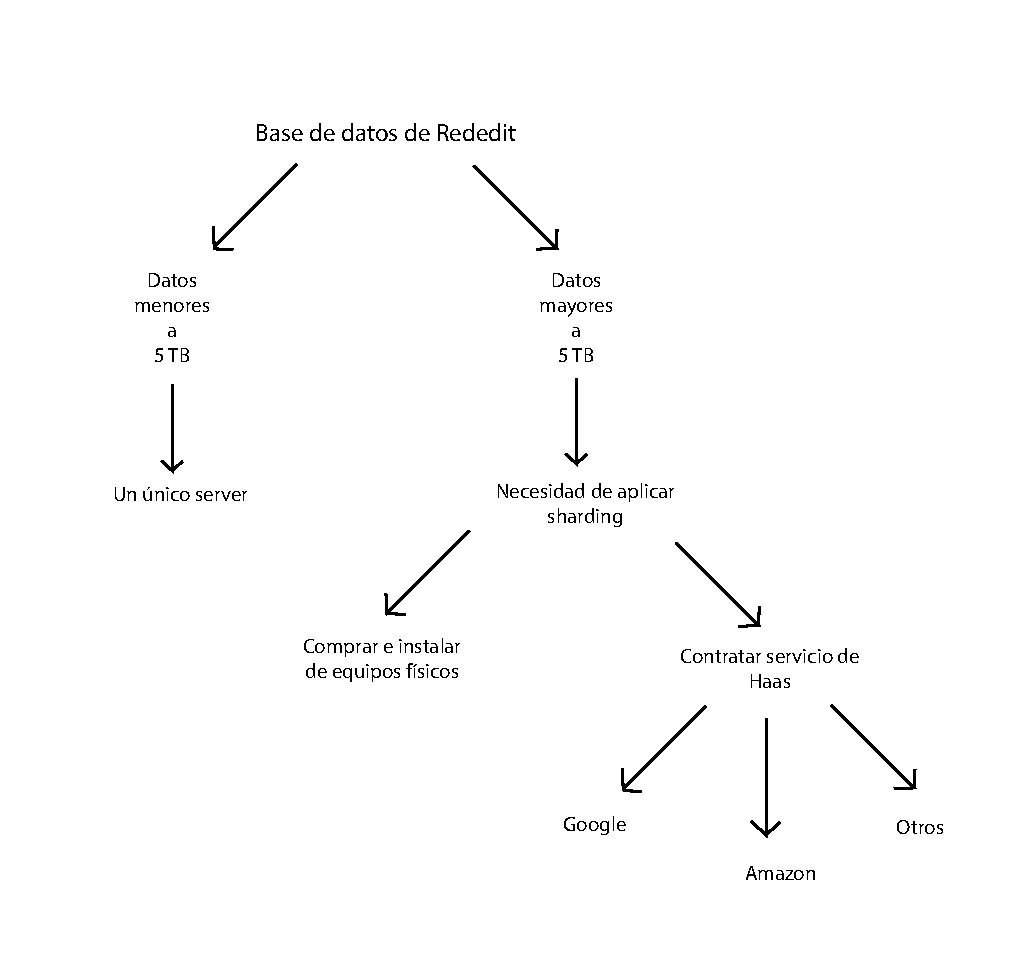
\includegraphics[keepaspectratio]{imagenes/im_1.pdf}
		  \caption{Cada nuevo par de juntas introduce 4 nuevas fuerzas}
		  \label{fig:contra1}
	\end{center}
\end{figure}
\FloatBarrier

\subsubsection{Sharding, conceptos generales}

''Sharding is the process of storing data records across multiple machines and is MongoDB’s approach to meeting the
demands of data growth. As the size of the data increases, a single machine may not be sufficient to store the data nor
provide an acceptable read and write throughput. Sharding solves the problem with horizontal scaling. With sharding,
you add more machines to support data growth and the demands of read and write operations.'' (MongoDB-sharding-guide)

''Vertical scaling adds more CPU and storage resources to increase capacity. Scaling by adding capacity has lim-
itations: high performance systems with large numbers of CPUs and large amount of RAM are disproportionately
more expensive than smaller systems. Additionally, cloud-based providers may only allow users to provision smaller
instances. As a result there is a practical maximum capability for vertical scaling.'' (MongoDB-sharding-guide)

''Sharding, or horizontal scaling, by contrast, divides the data set and distributes the data over multiple servers, or
shards. Each shard is an independent database, and collectively, the shards make up a single logical database.''

\subsubsection{Sharding en MongoDB}

''MongoDB supports sharding through the configuration of a sharded clusters.
Sharded cluster has the following components: shards, query routers and config servers. (MongoDB-sharding-guide)



